\documentclass[11pt,a4paper]{article}
\usepackage{fontspec}
\setmainfont{Latin Modern Roman}
\setmonofont{Latin Modern Mono}
\usepackage[margin=2.2cm]{geometry}
\usepackage{microtype}
\usepackage{amsmath,amssymb}
\usepackage{graphicx}
\usepackage{booktabs}
\usepackage{float}
\usepackage{caption}
\usepackage{hyperref}
\usepackage{xcolor}
\hypersetup{colorlinks=true,linkcolor=black,urlcolor=blue!50!black}
\graphicspath{{../Experimentos/graficos/}}
\setlength{\parskip}{4pt}
\setlength{\emergencystretch}{3em}
\renewcommand{\figurename}{Figura}
\renewcommand{\tablename}{Tabela}
\renewcommand{\contentsname}{Sumário}
\renewcommand{\refname}{Referências}

\title{Trabalho Prático: Divisão e Conquista\\\large Subarranjo de soma máxima e par de pontos mais próximos}
\author{Pedro Lemos \quad e \quad NOME DA DUPLA}
\date{Outubro de 2026}

\begin{document}
\maketitle

\section{Introdução}

Este relatório descreve a implementação e a análise de dois problemas resolvidos
por divisão e conquista (D\&C), cada um comparado com uma solução de força
bruta. Todo o código está em Python~3, no repositório
\url{https://github.com/pedrolems/DivisaoEConquista}, junto com os casos de
teste, os scripts de medição, os CSVs brutos e os gráficos aqui mostrados.

\section{Etapa 1: subarranjo de soma máxima}

Dado um vetor $A[1..n]$ de inteiros, procura-se o intervalo contínuo
$A[i..j]$ de maior soma. A saída é a soma e os índices $i$ e $j$.

\paragraph{Regra de desempate.} Quando dois intervalos têm a mesma soma,
escolhemos o que começa primeiro e, persistindo o empate, o mais curto.
A mesma função de comparação é usada nas três versões, o que garante que todas
devolvem exatamente o mesmo intervalo, inclusive nos empates.

\subsection{Força bruta}
Para cada início $i$, a soma é acumulada enquanto o fim $j$ avança, de modo que
cada intervalo é avaliado em $O(1)$. São $n(n+1)/2$ intervalos, logo
$T(n) = \Theta(n^2)$.

\subsection{Divisão e conquista}
O vetor é dividido ao meio; cada metade é resolvida recursivamente e, em seguida,
calcula-se o melhor subarranjo que cruza o meio: a melhor soma que termina em
$m$ (varrendo para a esquerda) somada à melhor soma que começa em $m+1$
(varrendo para a direita). Essa etapa percorre o trecho uma vez, em $\Theta(n)$.
A resposta é o melhor dos três candidatos. A recorrência é
\[
T(n) = 2\,T(n/2) + \Theta(n), \qquad T(1) = \Theta(1).
\]
Pelo caso 2 do Teorema Mestre ($a=2$, $b=2$, $f(n)=\Theta(n)=\Theta(n^{\log_2 2})$),
$T(n) = \Theta(n \log n)$. A árvore de recursão leva ao mesmo resultado: são
$\log_2 n$ níveis e cada nível realiza trabalho total $\Theta(n)$.

Para que o desempate seja respeitado, a combinação também precisa escolher bem
dentro de cada lado: na varredura para a esquerda, em caso de empate fica o
início mais à esquerda; na varredura para a direita, o fim mais próximo do
meio. Como a soma do intervalo cruzado é a soma das duas partes, que são
independentes, isso produz o intervalo cruzado com maior soma, menor início e
menor fim.

\subsection{Questão desafio: versão $O(n)$ (Kadane)}
Mantém-se a melhor soma de um intervalo que termina na posição atual. Ao chegar
em $A[k]$, se a soma acumulada for estritamente negativa ela é descartada e o
intervalo recomeça em $k$; se for zero, o intervalo é estendido, o que mantém o
início mais cedo exigido pelo desempate. Cada elemento é processado uma vez:
$T(n) = T(n-1) + \Theta(1) = \Theta(n)$.

\section{Etapa 2: par de pontos mais próximos}

Dados $n$ pontos no plano, procura-se o par com a menor distância euclidiana.
As distâncias são comparadas ao quadrado, sem raiz, para que coordenadas
inteiras sejam comparadas de forma exata.

\subsection{Força bruta}
Compara todos os $\binom{n}{2}$ pares: $T(n) = \Theta(n^2)$.

\subsection{Divisão e conquista}
Os pontos são ordenados uma única vez por $x$ ($P_x$) e por $y$ ($P_y$), com a
função \texttt{sorted} da biblioteca padrão, em $O(n \log n)$. Depois:
\begin{enumerate}
  \item \textbf{Dividir:} a primeira metade de $P_x$ forma o lado esquerdo e a
  segunda o lado direito; a linha vertical passa pela mediana $x_m$. A lista
  $P_y$ é separada nos dois lados em $O(n)$, mantendo a ordem por $y$ (marcamos
  os pontos do lado esquerdo e filtramos). Dividir pela posição em $P_x$, e não
  pelo valor de $x$, faz o algoritmo funcionar mesmo com muitos pontos de mesmo $x$.
  \item \textbf{Conquistar:} cada lado é resolvido recursivamente, e
  $\delta = \min(\delta_E, \delta_D)$.
  \item \textbf{Combinar:} a faixa contém os pontos com $|x - x_m| < \delta$,
  já ordenados por $y$. Cada ponto da faixa é comparado com no máximo os 7
  seguintes, parando antes se a diferença em $y$ já for $\ge \delta$.
\end{enumerate}
A combinação custa $\Theta(n)$ e a recorrência é a mesma da Etapa~1:
\[
T(n) = 2\,T(n/2) + \Theta(n) \;\Rightarrow\; T(n) = \Theta(n \log n),
\]
somada às duas ordenações iniciais, também $O(n \log n)$. O total é
$\Theta(n \log n)$.

\subsection{Por que bastam 7 comparações por ponto na faixa}
Seja $p$ um ponto da faixa. Os pontos que vêm depois de $p$ na ordem por $y$ e
que ainda podem estar a menos de $\delta$ de $p$ têm $0 \le y_q - y_p < \delta$
e $|x_q - x_m| < \delta$. Todos estão, portanto, no retângulo de largura
$2\delta$ e altura $\delta$ com base em $y_p$, centrado na linha divisória.

Esse retângulo é dividido em 8 quadrados de lado $\delta/2$: quatro do lado
esquerdo e quatro do lado direito da linha. Dois pontos dentro do mesmo
quadrado estariam a no máximo $\frac{\delta}{2}\sqrt{2} = \frac{\delta}{\sqrt2} < \delta$
um do outro. Mas cada quadrado fica inteiramente de um lado, e pontos do
mesmo lado estão a pelo menos $\delta$ um do outro, pela definição de $\delta$.
Logo cada quadrado tem no máximo um ponto, e o retângulo tem no máximo 8
pontos, contando o próprio $p$. Basta então comparar $p$ com os 7 pontos
seguintes. Os pontos anteriores a $p$ não precisam ser olhados, porque esses
pares já foram verificados quando o ponto anterior foi processado.

\subsection{Limiar}
Para subproblemas pequenos, a recursão tem custo fixo alto (criação de listas,
chamadas de função, montagem da faixa) e a força bruta é mais rápida. Por isso
a implementação usa um caso base híbrido: se o subproblema tem até
\texttt{LIMIAR} pontos, ele é resolvido por força bruta. A escolha do valor está
na Seção~\ref{sec:limiar}.

\section{Testes}

A bateria tem três partes:
\begin{itemize}
  \item \textbf{Testes unitários:} 34 testes, em
  \nolinkurl{EtapaUm/test_sub_soma_max.py} e
  \nolinkurl{EtapaDois/test_par_pontos_prox.py}, cada um com a
  justificativa na docstring. Cobrem os casos de borda do enunciado (vetor só
  com negativos, tamanho 1, empates) e outros que costumam quebrar
  implementações: só zeros, máximo no início ou no fim, intervalo que só aparece
  cruzando o meio, pontos repetidos, todos os pontos com o mesmo $x$ ou o mesmo
  $y$, par mais próximo cruzando a linha divisória, faixa com quase todos os
  pontos e coordenadas grandes.
  \item \textbf{Testes aleatórios:} 3000 vetores e 1500 conjuntos de pontos
  comparados com a força bruta. As faixas de valores são pequenas de
  propósito, para gerar muitos empates e pontos repetidos. Na Etapa~2 a D\&C é
  testada com limiar 1 (recursão até o fim, exercitando a faixa em todos os
  níveis), 3 e 16.
  \item \textbf{Casos em arquivo} (\texttt{Casos/}): 17 casos da Etapa~1 e 13
  da Etapa~2 no formato de entrada e saída do enunciado, com a justificativa de
  cada um em \texttt{Casos/README.md}. O script \texttt{rodar\_casos.py} executa
  todas as versões sobre cada caso (77 execuções, todas corretas).
\end{itemize}
Na Etapa~2, quando há mais de um par com a distância mínima, qualquer um é
aceito: o teste confere a distância e se o par devolvido realmente tem essa
distância.

\section{Metodologia experimental}

\begin{itemize}
  \item \textbf{Máquina:} Intel Xeon @ 2{,}80\,GHz, 2 núcleos (máquina virtual
  KVM), 7{,}8\,GiB de RAM, cache L3 de 33\,MiB, Linux 6.18 (Ubuntu 24.04),
  CPython 3.13.18 (arquivo \texttt{Experimentos/maquina.txt}).
  \item \textbf{Tamanhos:} $n = 100, 200, 400, 800, 1600, 3200, 6400$, com 5
  execuções por tamanho. Cada execução usa uma entrada aleatória diferente
  (semente fixa), e a mesma entrada é usada por todos os algoritmos da etapa.
  Vetores com valores em $[-1000, 1000]$; pontos com coordenadas inteiras em
  $[0, 10^6]$.
  \item \textbf{Medição:} \texttt{time.perf\_counter} em volta da chamada da
  função, sem contar leitura de entrada nem geração dos dados. Na Etapa~2 o
  tempo da D\&C inclui as ordenações iniciais.
  \item \textbf{Dados brutos:} \texttt{Experimentos/medicoes.csv} (todas as
  execuções), \texttt{limiar.csv} e \texttt{pequenos.csv}.
\end{itemize}

\section{Resultados e discussão}

\subsection{Etapa 1}

\begin{table}[H]
\centering\small
\begin{tabular}{rrrr}
\toprule
$n$ & Força bruta (ms) & D\&C (ms) & Kadane (ms) \\
\midrule
100  & 0{,}739 $\pm$ 0{,}085 & 0{,}226 $\pm$ 0{,}005 & 0{,}020 $\pm$ 0{,}001 \\
200  & 2{,}894 $\pm$ 0{,}172 & 0{,}514 $\pm$ 0{,}060 & 0{,}037 $\pm$ 0{,}001 \\
400  & 15{,}681 $\pm$ 3{,}590 & 1{,}327 $\pm$ 0{,}403 & 0{,}088 $\pm$ 0{,}024 \\
800  & 49{,}060 $\pm$ 2{,}924 & 2{,}491 $\pm$ 0{,}671 & 0{,}160 $\pm$ 0{,}050 \\
1600 & 199{,}245 $\pm$ 12{,}874 & 4{,}650 $\pm$ 0{,}083 & 0{,}275 $\pm$ 0{,}013 \\
3200 & 776{,}275 $\pm$ 23{,}010 & 10{,}033 $\pm$ 0{,}249 & 0{,}601 $\pm$ 0{,}074 \\
6400 & 3198{,}061 $\pm$ 164{,}467 & 21{,}366 $\pm$ 0{,}881 & 1{,}189 $\pm$ 0{,}141 \\
\bottomrule
\end{tabular}
\caption{Etapa 1: tempo médio $\pm$ desvio padrão de 5 execuções.}
\end{table}

\begin{figure}[H]
\centering
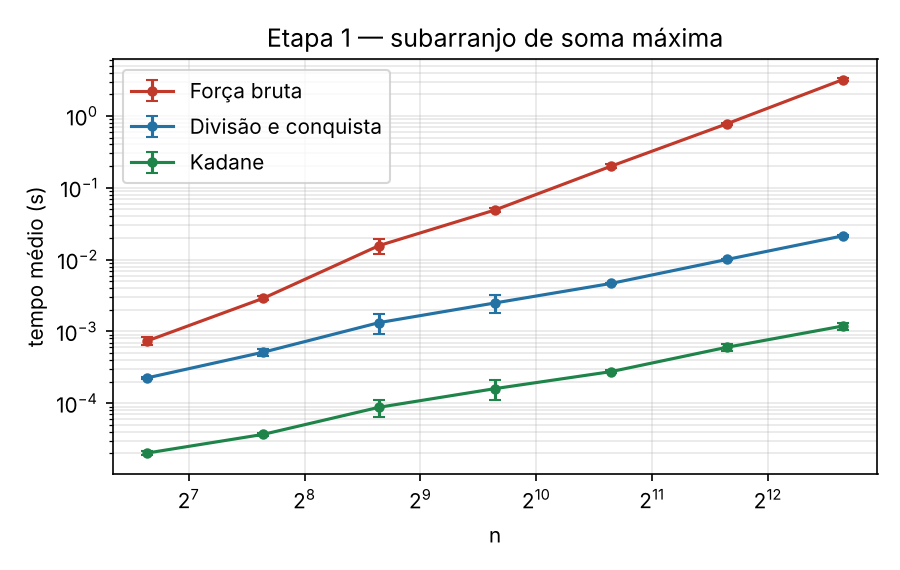
\includegraphics[width=0.49\textwidth]{etapa1_tempos.png}
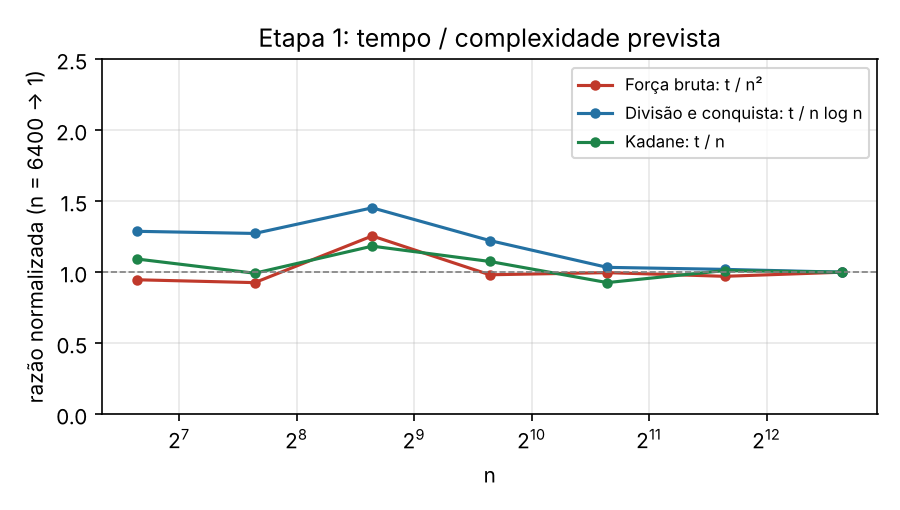
\includegraphics[width=0.49\textwidth]{etapa1_razao.png}
\caption{Etapa 1. Esquerda: tempo em escala log-log. Direita: tempo dividido
pela complexidade prevista, normalizado para valer 1 em $n=6400$.}
\end{figure}

No gráfico log-log, uma função $c\,n^k$ aparece como uma reta de inclinação $k$.
O ajuste por mínimos quadrados deu inclinação \textbf{2{,}00} para a força
bruta, \textbf{1{,}07} para a D\&C e \textbf{0{,}98} para Kadane. A força bruta
e Kadane batem com $n^2$ e $n$. Para $n \log n$ a inclinação esperada nessa
faixa fica um pouco acima de 1, já que $\log n$ cresce devagar: entre $n=100$ e
$n=6400$ o fator $\log_2 n$ passa de 6{,}6 para 12{,}6, o que soma cerca de
0{,}15 à inclinação. O valor medido, 1{,}07, está dentro do esperado.

O gráfico da direita é um teste mais direto: se o tempo segue a complexidade
prevista, $t/f(n)$ é constante. As três curvas ficam perto de 1, com desvios
maiores apenas nos tamanhos menores, em que os tempos estão abaixo de 1\,ms e
pesam mais os custos fixos e as variações do sistema. Em $n=400$ há um pico nas
três curvas que coincide com o maior desvio padrão da tabela; como aparece em
algoritmos diferentes, é ruído da máquina virtual e não do algoritmo.

Em $n=6400$, a D\&C é cerca de 150 vezes mais rápida que a força bruta, e Kadane
cerca de 2700 vezes. A cada duplicação de $n$, o tempo da força bruta
multiplica por aproximadamente 4, o da D\&C por um pouco mais de 2 e o de Kadane
por 2.

\subsection{Etapa 2}

\begin{table}[H]
\centering\small
\begin{tabular}{rrr}
\toprule
$n$ & Força bruta (ms) & D\&C, limiar 16 (ms) \\
\midrule
100  & 1{,}434 $\pm$ 0{,}087 & 0{,}411 $\pm$ 0{,}181 \\
200  & 5{,}333 $\pm$ 0{,}235 & 1{,}578 $\pm$ 1{,}881 \\
400  & 27{,}497 $\pm$ 4{,}079 & 2{,}332 $\pm$ 0{,}851 \\
800  & 108{,}031 $\pm$ 20{,}511 & 3{,}814 $\pm$ 0{,}470 \\
1600 & 403{,}691 $\pm$ 21{,}532 & 9{,}032 $\pm$ 1{,}925 \\
3200 & 1625{,}689 $\pm$ 68{,}505 & 16{,}549 $\pm$ 0{,}166 \\
6400 & 6687{,}525 $\pm$ 202{,}613 & 39{,}890 $\pm$ 5{,}148 \\
\bottomrule
\end{tabular}
\caption{Etapa 2: tempo médio $\pm$ desvio padrão de 5 execuções.}
\end{table}

\begin{figure}[H]
\centering
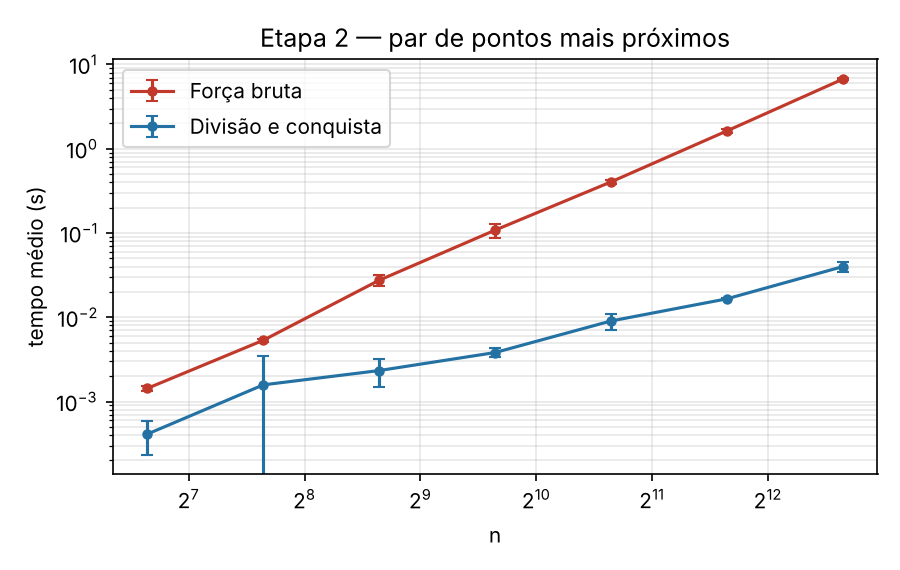
\includegraphics[width=0.49\textwidth]{etapa2_tempos.png}
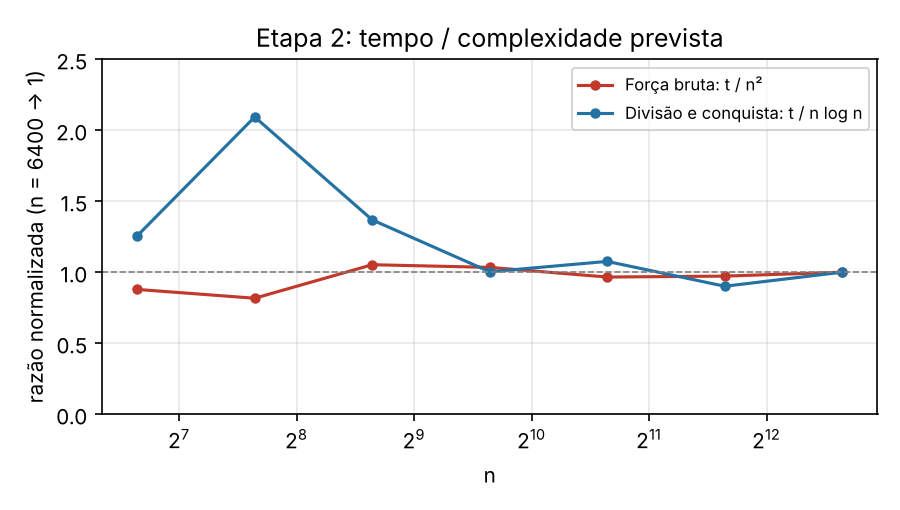
\includegraphics[width=0.49\textwidth]{etapa2_razao.png}
\caption{Etapa 2. Esquerda: tempo em escala log-log. Direita: tempo dividido
pela complexidade prevista, normalizado para valer 1 em $n=6400$.}
\end{figure}

As inclinações ajustadas foram \textbf{2{,}03} para a força bruta e
\textbf{1{,}02} para a D\&C, de novo de acordo com $n^2$ e $n \log n$. A razão
$t/n^2$ da força bruta fica entre 0{,}8 e 1{,}05 em toda a faixa. A razão
$t/(n\log n)$ da D\&C estabiliza a partir de $n=800$; o ponto fora da curva em
$n=200$ vem de uma única execução lenta (o desvio padrão, 1{,}9\,ms, é maior que
a própria média), provavelmente uma pausa do coletor de lixo ou da máquina
virtual. Por isso o CSV guarda as execuções individuais. Em $n=6400$ a D\&C é
cerca de 170 vezes mais rápida.

A D\&C da Etapa~2 é um pouco mais lenta que a da Etapa~1 para o mesmo $n$
(40\,ms contra 21\,ms em $n=6400$), embora as duas sejam $\Theta(n\log n)$:
cada nível da recursão monta listas novas e calcula distâncias com tuplas,
enquanto a Etapa~1 só soma inteiros. As constantes mudam; o crescimento não.

\subsection{Quando cada abordagem vence}

\begin{figure}[H]
\centering
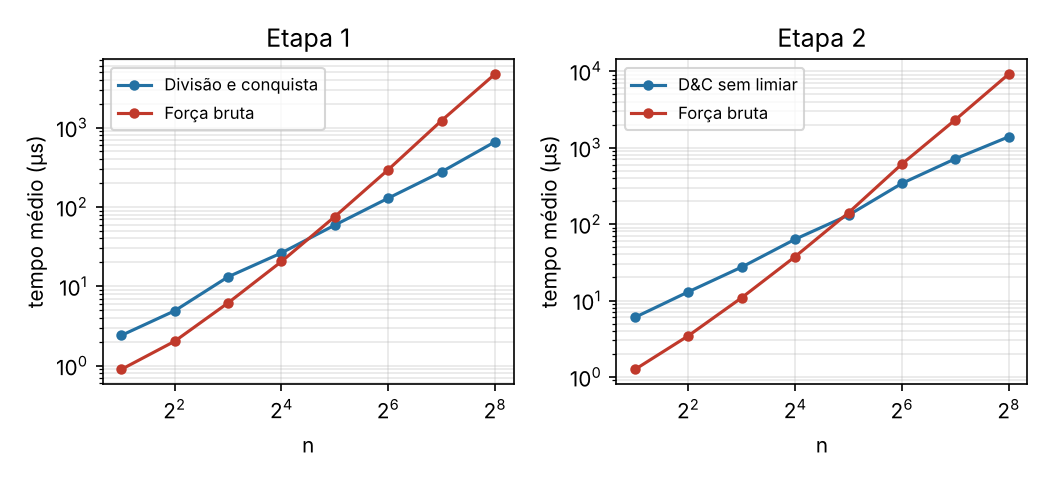
\includegraphics[width=0.75\textwidth]{pequenos.png}
\caption{Tamanhos pequenos (média de 5 medições, cada uma com 200 execuções).
Na Etapa 2 a D\&C roda sem limiar, com a recursão indo até 1 ponto.}
\end{figure}

Para $n$ pequeno a força bruta vence nas duas etapas. Na Etapa~1, com $n=8$, ela
leva 6\,\textmu s contra 13\,\textmu s da D\&C; na Etapa~2, 11\,\textmu s contra
27\,\textmu s. A explicação está nas constantes. A força bruta é formada por
laços simples, sem chamadas de função nem alocação. A D\&C, em cada chamada,
cria listas, faz chamadas recursivas e percorre a faixa; com poucos elementos
esse custo fixo domina e não há ganho que compense.

O cruzamento acontece entre $n=16$ e $n=32$ nas duas etapas. Acima disso o
fator $n$ contra $\log n$ passa a dominar e a diferença cresce rápido: em
$n=256$ a D\&C já é 7 vezes mais rápida na Etapa~1 e 6{,}6 vezes na Etapa~2.
Kadane vence em todos os tamanhos, porque tem a menor complexidade e também
as menores constantes (um único laço).

\subsection{Escolha do limiar da Etapa 2}\label{sec:limiar}

\begin{figure}[H]
\centering
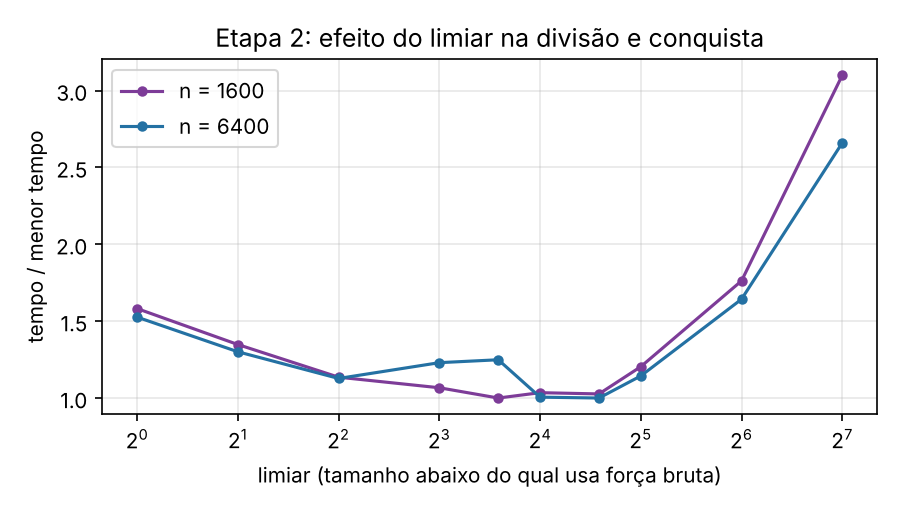
\includegraphics[width=0.62\textwidth]{etapa2_limiar.png}
\caption{Tempo da D\&C da Etapa 2 em função do limiar, dividido pelo menor
tempo de cada tamanho (5 execuções por ponto).}
\end{figure}

\begin{table}[H]
\centering\small
\begin{tabular}{rrrrrrrrrrr}
\toprule
limiar & 1 & 2 & 4 & 8 & 12 & 16 & 24 & 32 & 64 & 128 \\
\midrule
$n=1600$ (ms) & 11{,}4 & 9{,}7 & 8{,}2 & 7{,}7 & 7{,}2 & 7{,}4 & 7{,}4 & 8{,}6 & 12{,}7 & 22{,}2 \\
$n=6400$ (ms) & 56{,}6 & 48{,}3 & 41{,}8 & 45{,}6 & 46{,}3 & 37{,}3 & 37{,}1 & 42{,}4 & 60{,}9 & 98{,}6 \\
\bottomrule
\end{tabular}
\caption{Tempo médio da D\&C da Etapa 2 para cada limiar.}
\end{table}

O limiar afeta o tempo de duas formas opostas. Se é pequeno demais, a recursão
desce até subproblemas de 1 ou 2 pontos, em que o custo fixo de cada chamada
domina: com limiar 1 o tempo é cerca de 50\% maior que o melhor. Se é grande
demais, a força bruta passa a trabalhar em subproblemas grandes, onde o custo
quadrático pesa: com limiar 128 o tempo é 2{,}7 a 3 vezes o melhor. Entre esses
extremos há uma região plana, aproximadamente de 12 a 24, em que as diferenças
ficam dentro do ruído das medições.

Escolhemos \textbf{limiar 16}, que está no centro dessa região para os dois
tamanhos medidos. O valor é coerente com o experimento da seção anterior, em
que a força bruta deixa de ser mais rápida entre 16 e 32 pontos: abaixo do
cruzamento compensa usar a força bruta, e acima dele compensa continuar
dividindo. Escolher um valor no centro da região plana, e não exatamente o
mínimo medido, deixa a escolha menos sensível ao ruído e a variações entre
máquinas. O limiar não muda a complexidade assintótica: com limiar constante
$L$, as folhas custam $O(L^2)$ cada e há $O(n/L)$ delas, o que dá $O(nL)$, ainda
$O(n)$ para $L$ fixo.

\section{Conclusão}

As medições confirmaram as complexidades previstas pelas recorrências: as
inclinações em escala log-log ficaram em 2{,}00 e 2{,}03 para as forças brutas,
1{,}07 e 1{,}02 para as versões D\&C (compatíveis com $n\log n$) e 0{,}98 para
Kadane, e as razões tempo/complexidade ficaram aproximadamente constantes. A
força bruta só vence para entradas muito pequenas, abaixo de 16 a 32 elementos,
por ter constantes menores; esse mesmo ponto de cruzamento orientou a escolha
do limiar 16 no caso base híbrido da Etapa~2. Para os tamanhos maiores medidos,
as versões D\&C foram de 150 a 170 vezes mais rápidas, e o algoritmo linear de
Kadane mostra que, na Etapa~1, ainda é possível ir além da divisão e conquista.

\end{document}
